\chapter{Fundamentarea teoretică și soluții similare}
\label{cap:cap2}

\section{VR / AR}

Realitatea virtuală și-a făcut apariția conceptuală și experimentală pentru prima dată în anul 1968, odată cu dispozitivul creat de Ivan Sutherland și Bob Sproull, considerat primul sistem de afișare „head-mounted” (HMD). Acest sistem era conectat la un calculator mainframe al epocii, care ocupa adesea o întreagă încăpere și era singurul capabil să proceseze și să redea imaginile grafice tridimensionale simple necesare. Dispozitivul HMD în sine era greoi, impunând suspendarea de tavan, fapt ce i-a atras porecla „The Sword of Damocles” și a subliniat limitările hardware considerabile ale acelor timpuri.

\begin{figure}[h!]
    \centering
    \begin{subfigure}{0.49\textwidth}
        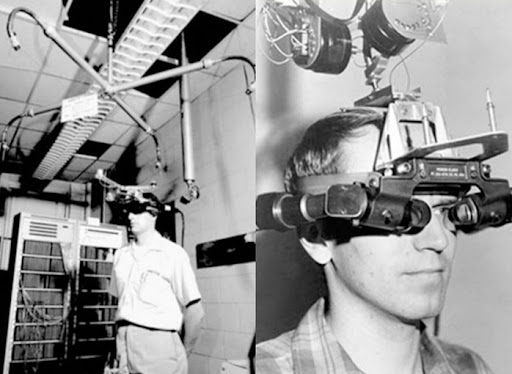
\includegraphics[width=\linewidth, height=6cm]{continut/capitol2/figuri/sword_of_damocles.jpg}
        \caption{The Sword of Damocles}
        \label{fig:sword_of_damocles}
    \end{subfigure}
    \hfill
    \begin{subfigure}{0.49\textwidth}
        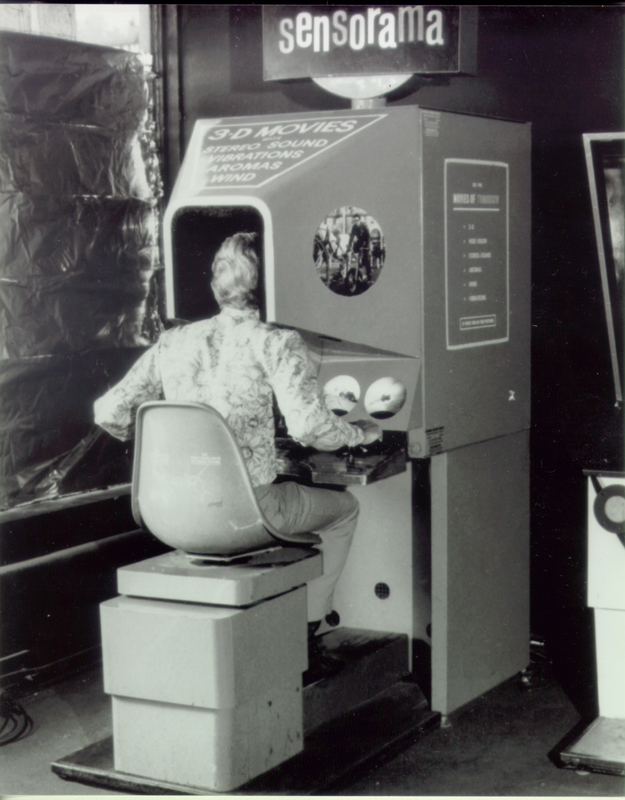
\includegraphics[width=\linewidth, height=6cm]{continut/capitol2/figuri/sensorama.jpg}
        \caption{The Sensorama}
        \label{fig:sensorama}
    \end{subfigure}

    \caption{Istoria VR: Dispozitive timpurii}
    \label{fig:VR_history}
\end{figure}


Desigur, au existat și concepte anterioare acestei inovații. Un exemplu notabil este Sensorama, inventat de Morton Heilig în 1957. Această mașinărie electromecanică voluminoasă funcționa ca o unitate autonomă, integrând toate componentele necesare pentru a oferi o experiență multisenzorială (imagini 3D, sunet stereo, mirosuri, vibrații) pentru până la patru persoane simultan. 
Deși nu era un HMD și nu necesita un calculator extern în sensul modern, Sensorama a reprezentat un precursor important al experiențelor imersive, demonstrând potențialul stimulării multiplelor simțuri.
\begin{wrapfigure}{r}{5cm}
    \centering
    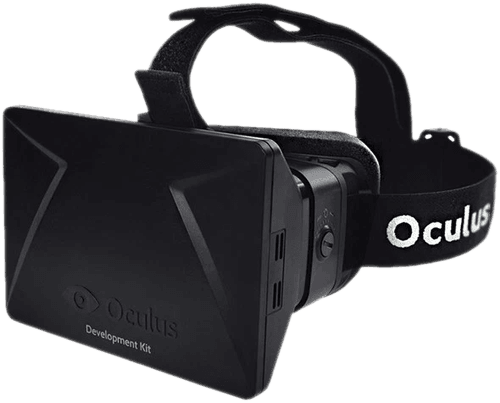
\includegraphics[width=5cm]{continut/capitol2/figuri/oculusriftdk1.png}
    \caption{Oculus Rift DK1}
    \label{fig:Oculus_DK1}
\end{wrapfigure}
Trecerea de la experimente academice la produse orientate către consumatori a fost marcată decisiv de lansarea primului dispozitiv VR fabricat în masă și disponibil publicului larg: Oculus Rift DK1, în martie 2013, la un preț de aproximativ 300 de dolari (aproximativ 450\$ în anul 2025, după calcularea inflației). Apariția sa a fost strâns legată de progresele în tehnologia ecranelor compacte de înaltă rezoluție (impulsionate de industria telefoanelor mobile) și, crucial, de creșterea exponențială a puterii de calcul și accesibilității computerelor personale (PC-urilor). 
Aceste PC-uri, echipate cu plăci grafice din ce în ce mai performante, au devenit platforma hardware necesară pentru a rula aplicațiile VR. Kitul de dezvoltare Oculus Rift DK1 oferea un ecran de 7 inch (1280x800 px, rezultând 640x800 px per ochi), un câmp vizual de aproximativ 90 de grade și un sistem de urmărire a mișcării capului pe trei axe (head-tracking). Deși nu oferea urmărire a poziției în spațiu (positional tracking), care a devenit un standard ulterior și a necesitat dezvoltarea unor sisteme de senzori suplimentari (externi sau integrați), DK1 a reprezentat un moment cheie în popularizarea realității virtuale.
De atunci, evoluția hardware-ului VR a continuat într-un ritm alert.
Dispozitivele ulterioare au adus îmbunătățiri semnificative: rezoluții mult mai mari ale ecranelor, câmpuri vizuale extinse, rate de reîmprospătare superioare, sisteme de urmărire pozițională din ce în ce mai precise (inside-out tracking, eliminând nevoia senzorilor externi), și controlere dedicate cu feedback haptic. În paralel, cerințele hardware pentru PC-urile capabile să susțină aceste experiențe au rămas ridicate, dar au apărut și soluții alternative: console de jocuri cu suport VR și, mai recent, dispozitive VR autonome (standalone), care integrează unitatea de procesare direct în cască, eliminând dependența de un PC sau o consolă externă.

Fie că vorbim despre un dispozitiv VR lansat recent sau unul istoric, principiul de funcționare a rămas același: simularea unei alte realități prin intermediul unor afișaje dedicate pentru fiecare ochi, însoțite de sunet stereo sau 3D, livrat prin căști sau boxe speciale. Cu ajutorul acestor elemente hardware esențiale, simțurile noastre sunt „păcălite” să creadă că ne aflăm într-un alt spațiu, în afara realității imediate, oferind o senzație intensă de imersiune.

\section{Unreal Engine 5}

Fiind succesorul lui Unreal Engine 4, Unreal Engine 5 (UE5) este un motor de joc („game engine”) care permite realizarea unor experiențe interactive de ultimă generație, fiind mult mai ușor de folosit decât dezvoltarea unui engine de la zero. Punctul de plecare este același pentru toți dezvoltatorii, însă UE5 oferă o infinitate de direcții și domenii spre care aceștia se pot orienta. În majoritatea cazurilor sunt create jocuri, dar există și numeroase exemple extra-ludice în care motorul este extrem de util.

\begin{figure} [htp] 
\centering 
\includegraphics [width=12cm]
{continut/capitol2/figuri/ue5.png} 
\caption{Unreal Engine 5 - Deschiderea proiectului} 
\label{fig:VR} 
\end{figure}


Spre exemplu, BMW, Audi, Porsche și Volvo folosesc Unreal pentru dezvoltarea de simulări și prezentări interactive în showroom-uri virtuale: testează noile modele în medii digitale, simulează experiența de condus și rafinează designul auto. Scene din serialul The Mandalorian sau din demonstrația tehnologică The Matrix Awakens se bazează pe UE5 pentru efecte speciale și decoruri realiste, economisind astfel cheltuieli semnificative legate de recuzită fizică.

Versiunea majoră 5.0 (lansată pe 5 aprilie 2022) a adus numeroase îmbunătățiri - Nanite (sistem de geometrie pe bază de micro-poligoane), Lumen (iluminare globală și reflexii în timp real), Ray Tracing avansat, optimizări de performanță și flux de lucru, suport extins pentru MetaHuman și un sistem modernizat de animație și simulare fizică.

Noutățile din 5.4 (folosită în proiectul VR Museum):

\begin{adjustwidth}{2em}{0pt}
\begin{description}
    \item[\textbf{Suport VR/AR unificat prin OpenXR: }] În locul mai multor plugin-uri specifice (de ex. Oculus Plugin pentru Meta Quest), OpenXR oferă un cadru universal compatibil cu majoritatea headset-urilor, reducând timpul de configurare a aceleiași scene pe platforme diferite.
    \item[\textbf{{World Partition: }}] Permite împărțirea lumii în sectoare încărcate și descărcate dinamic, optimizând proiectele cu hărți mari și îmbunătățind performanța editorului și a build-ului final.
    \item[\textbf{{Motion Matching \& animație dinamică avansată: }}] Motorul înțelege mult mai bine părțile corpului și tranzițiile lor, facilitând crearea de animații realiste într-un timp redus. Tehnologia folosește o bază de date de mișcări care sunt selectate și combinate automat în funcție de contextul de gameplay.
\end{description}
\end{adjustwidth}

\section{Ray Tracing}

În jocurile de acum câțiva ani se foloseau diverse tehnici de calculare a luminii. De obicei, lumina era atașată unor obiecte definite drept „light objects”. Parcursul razei era trasat de la punctul A (obiectul emitent) până la punctul B (primul obstacol — un perete ori alt obiect 3D). Din punct de vedere vizual, această metodă tradițională arată în continuare foarte bine datorită optimizărilor și evoluției algoritmilor de rasterizare; totuși, din perspectiva realismului există limite evidente.

Aici intervine Ray Tracing-ul în timp real. Spre deosebire de metodele clasice, tehnica simulează comportamentul fizic al luminii din lumea reală:

\begin{itemize}
    \item Lumina pornește din sursa emitentă în toate direcțiile.
    \item Razele se reflectă, refractă sau sunt absorbite diferit, în funcție de proprietățile fiecărui material (culoare, rugozitate, indice de refracție).
    \item Obiectele din scenă sunt iluminate atât direct (de la sursa primară), cât și indirect (prin reflexii multiple sau lumină difuză), creând umbre moi, reflexii precise și o iluminare globală mai verosimilă.
\end{itemize}

Tehnologia Ray Tracing nu este nouă; ea este folosită de mult timp în cinematografie, mai ales în filmele de animație 3D produse de studiouri precum Pixar, DreamWorks sau Disney. În producția de film, fiecare cadru poate fi randat în minute ori chiar ore pe multe servere, unde costul nu este constrâns de cerințe de timp real. Din acest motiv, tehnica era considerată impracticabilă pentru jocurile video: hardware-ul existent putea livra doar 2–5 cadre pe secundă în condiții optime, mult sub pragul necesar pentru un gameplay fluent.


\section{Evoluția hardware}

Acest lucru s-a schimbat în anul 2018, când Nvidia a lansat prima serie de plăci video ce pot simula lumina în timp real, seria RTX 20. Aceste placi video aveau cateva imbunatatiri fata de seria precedenta, GTX 16: Noi nuclee RT făcute special pentru Ray Tracing, nuclee Tensor pentru DLSS, mult mai multe nuclee CUDA, memorie mai rapidă și shadere Mesh, folosite pentru a susține geometrie mult mai avansată și complexă fără a pierde din perfomanta.

În mod normal, un joc (sau în cazul nostru, o experiență VR) trebuie să ruleze cu peste 30 fps pentru claritate și cu peste 60 fps pentru o experiență cu adevărat plăcută ochilor. Abia odată cu apariția plăcilor grafice cu nuclee dedicate pentru ray tracing și a tehnicilor de upscaling inteligente (DLSS, FSR) a devenit posibilă integrarea ray tracing-ului în timp real, păstrând totodată un număr suficient de cadre pe secundă pentru jocuri moderne.

\section{\textbf{D}eep \textbf{L}earning \textbf{S}uper \textbf{S}ampling}

Prescurtat DLSS și avand 4 versiuni în momentul actual, acest algoritm folosește nucleele Tensor pentru a spori calitatea imaginii. jocul este randat la o rezolutie mai mica, iar placa video tehnologia DLSS pentru a face “upscaling” la imagine, astfel permitandu-ne sa jucam la setari grafice mult mai mari și desigur, cu Ray Tracing pornit.

Cele patru mari generații sunt: 

\begin{center}
\begin{tabular}{||c c c||} 
 \hline
 Versiune & Anul lansării & Noile funcții introduse \\ [0.5ex] 
 \hline\hline
 DLSS 1.0 & 2018 & Super-Sampling AI clasic \\ 
 \hline
 DLSS 2.0 & 2020 & Super Temporal Resolution \\
 \hline
 DLSS 3 & 2022 & Frame Generation, cadre AI pe seria RTX 40 \\
 \hline
 DLSS 4 & 2025 & Multi Frame Generation, mai multe cadre AI generate \\ [1ex] 
 \hline
\end{tabular}
\end{center}

\noindent Între acestea, DLSS 3.5 (2023) a adus „Ray Reconstruction”, un nou model AI care înlocuiește denoiser-ele clasice pentru reflexii și iluminare ray-traced. 

Prima evoluție s-a intamplat în anul 2020 când Nvidia a lansat seria de plăci video RTX 30, unde și-a făcut apariția DLSS 2. Acesta nu numai ca este mult mai eficient și antrenat pe un model mai performant, ci are 4 noi setari: 

\begin{center}
\begin{tabular}{||c c||} 
 \hline
 Calitatea DLSS & Rezoluția internă (procent) \\ [0.5ex] 
 \hline\hline
 Ultra Performance & 33\% (Introdus in DLSS 2.1) \\ 
 \hline
 Performance & 50\%  \\
 \hline
 Balanced & 58\% \\
 \hline
 Quality & 66.6\%  \\ [1ex] 
 \hline
 Native Upscale & 100\% (DLAA, introdus in DLSS 2.2)  \\ [1ex] 
 \hline
\end{tabular}
\end{center}


 În 2022, odată cu seria GeForce RTX 40, DLSS 3 a extins aceste moduri cu Frame Generation, multiplicând rata de cadre cu 2-3× pe titluri compatibile (de ex. Cyberpunk 2077 RT Overdrive). În 2025, DLSS 4 duce mai departe ideea prin Multi Frame Generation, generând până la 8× mai multe cadre la 4K pe RTX 5090, cu un nou model transformator ce îmbunătățește stabilitatea temporală și reduce ghosting-ul. 

Dacă jocul este randat la 1080p (1920×1080), rezoluția reală înainte de acest “upscale” realizat de DLSS sunt următoarele: 

\begin{center}
\begin{tabular}{||c c||} 
 \hline
 Calitatea DLSS & Rezoluția internă \\ [0.5ex] 
 \hline\hline
 Ultra Performance & 640×360 \\ 
 \hline
 Performance & 960×540  \\
 \hline
 Balanced & 1114×626 \\
 \hline
 Quality & 1280×720  \\ [1ex] 
 \hline
 Native Upscale & 1920x1080 \\ [1ex] 
 \hline
\end{tabular}
\end{center}


\noindent Aspectual, deși jocul este la o rezoluție mult mai mică, nu arată foarte diferit față de rezoluția “native”, atunci când nu ar fi fost folosit DLSS. Singurele diferențe se pot remarca la modurile Ultra Performance și Performance la mișcări bruște ale camerei, în special când ne uitam la margini (ex: frunzele din copaci în raport cu cerul, etc.)

DLSS păstrează aceeași factori de scalare pentru 1440p și 4K, iar Ray Reconstruction (DLSS 3.5+) poate diminua artefactele de la margini în scene ray-traced, chiar și în modurile cu rezoluție internă foarte mică. De asemenea, tehnologia poate fi combinată cu NVIDIA Reflex pentru a reduce latența de intrare la sub 10 ms în titluri competitive.

\section{Nanite}

Tehnologia Nanite a fost lansată în anul 2020 împreună cu Unreal Engine 5. Aceasta permite scene vizuale mult mai detaliate, fără a afecta performanța. Dacă pană atunci developerii erau nevoiți sa optimizeze manual numărul de poligoane ce alcătuiau obiectele, după apariția noii tehnologii nu a mai fost necesar. 

Cu Nanite, obiectele, texturile, nivelul de detaliu este ajustat dinamic în funcție de distanța jucătorului pana la obiect, unghiul vizual și puterea de procesare a calculatorului. Astfel, pe ecran va fi reprezentat exact nivelul necesar de poligoane, nu mai mult, nici mai puțin.

\section{Lumen}

Apărut odată cu Unreal Engine 5 și cu Nanite, tehnologia Lumen simuleaza lumina în timp real prin folosirea unor tehnici foarte optimizare.

\textbf{Care este diferenta intre Lumen și Ray Tracing?}

Spre deosebire de Ray Tracing ce folosește nucleele RT pentru procesarea luminii, tehnologia Lumen folosește o combinație dintre \textbf{Voxel Cone Tracing}, \textbf{Global Illumination} si \textbf{Screen Space Reflections} (sau prescurtat SSR) pentru a face posibilă utilizarea și pe un hardware de nivel mediu. 

\begin{adjustwidth}{2em}{0pt}
\begin{description}
    \item[\textbf{Voxel Cone Tracing:}] scena este convertită într-un set de voxels. Acestea se aseamănă cu pixelii, însă în loc de o reprezentare de culoare pe un  plan bidimensional, aceste voxels sunt realizate în spațiul 3D și au mai multe proprietăți (densitate, transparenta, etc.) 
    \item[\textbf{Global Illumination:}] Folosește metoda Ray Tracing pentru a reprezenta un ambient cat mai similar cu lumea reala in ceea ce privește trasarea razelor de lumina.
    \item[\textbf{Screen Space Reflections:}] tehnologie folosită tradițional, nu foarte costisitoare, unde reflexia era generată în funcție de conținutul pe ecran. In general folosita pe suprafete mari (spre exemplu apa), aceasta nu era foarte costisitoare, însă se putea observa cu usurinta folosirea acestei tehnologii prin mișcarea unghiului camerei.
\end{description}
\end{adjustwidth}

\noindent Lumen poate fi folosit și cu Ray Tracing la nivel hardware, pentru un nivel de detaliu mai avansat fără a afecta performanța atat de mult fata de Ray Tracing standard.







\section{Soluții și proiecte asemănătoare}

Dacă ne uităm la exemple din afara țării, putem identifica câteva soluții mai mult sau mai puțin asemănătoare cu VR Museum.

Unul dintre cele mai cunoscute este Google Arts \& Culture, lansat în 2011, un proiect ambițios care oferă tururi virtuale ale peste 500 de muzee din întreaga lume. Experiența este disponibilă atât pe web, cât și în aplicații mobile, iar unele dintre muzeele prezentate sunt compatibile cu dispozitive VR pentru telefon, cum ar fi Google Cardboard. Interacțiunea este însă limitată la explorare vizuală prin imagini 360°, fără posibilități avansate de interacțiune cu obiectele sau mediul.

Un alt exemplu relevant este The Glass Drawing Room – Corning Museum of Glass. Acest proiect, realizat în Unity și inspirat de viziunea arhitectului Robert Adam, recreează în VR o cameră de desen din secolul al XVIII-lea. Sunt puse în evidență detalii precum oglinzile, panourile decorative din sticlă și atmosfera generală a epocii. Aplicația este disponibilă gratuit pentru descărcare.

De asemenea, proiectul Digital Homecoming, realizat de Technology Research Institute for Culture \& Heritage (TRIC), folosește Unreal Engine, același motor grafic utilizat și în dezvoltarea VR Museum. Proiectul creează replici digitale ale artefactelor culturale coreene și le prezintă în expoziții interactive, accesibile publicului din Coreea de Sud și Statele Unite ale Americii. Acesta evidențiază potențialul realității virtuale în conservarea și promovarea patrimoniului cultural.

\section{Cum se construiește o experiență virtuală?}

În ceea ce privește o experiență de tip Virtual Reality, aceasta poate fi realizată în mai multe moduri, în funcție de buget, nivelul dorit de interactivitate și scopul aplicației.

Cea mai accesibilă variantă implică utilizarea unui telefon mobil introdus într-un set de ochelari VR pasivi (precum Google Cardboard), care măresc ecranul telefonului și oferă o experiență de vizualizare 360°. Din păcate, această metodă oferă un control limitat și un nivel redus de realism, fără interacțiune reală cu mediul virtual.

La polul opus, cea mai performantă variantă implică utilizarea unui headset VR dedicat, dotat cu ecran pentru fiecare ochi și controlere pentru interacțiune (ex: Meta Quest 2, folosit și în cadrul acestui proiect). Aceste dispozitive permit urmărirea poziției capului și a mâinilor, oferind o experiență complet imersivă și interactivă.

Realizarea unui astfel de proiect necesită însă timp, experiență și, de cele mai multe ori, o echipă de dezvoltare, pentru a putea livra o aplicație la un nivel consumer-ready. De aceea, multe aplicații VR comerciale sunt disponibile contra cost. În schimb, în mediul educațional și științific, proiectele sunt adesea gratuite, pentru a asigura accesul larg la informații.

Aplicațiile VR pot fi clasificate în mai multe categorii:

\begin{adjustwidth}{2em}{0pt}
\begin{description}
    \item[\textbf{Experiențe 360°}] - bazate pe fotografii sau videoclipuri sferice, unde utilizatorul se poate uita în jur, dar nu poate interacționa sau deplasa;    
    \item[\textbf{Experiențe interactive}] - unde utilizatorul se poate mișca liber în spațiul virtual și poate interacționa cu obiectele din jurul său.
\end{description}
\end{adjustwidth}

\noindent În ceea ce privește nivelul de realism grafic, aplicațiile VR pot fi împărțite în două mari categorii:

\begin{adjustwidth}{2em}{0pt}
\begin{description}
    \item[\textbf{Experiențe cu grafică simplificată}] - create cu resurse reduse (adesea în Unity sau pe console standalone);   
    \item[\textbf{Experiențe avansate}] conectate la un PC cu placă grafică dedicată, unde procesarea este realizată pe computer, iar imaginea este transmisă către headset-ul VR prin cablu sau wireless.
\end{description}
\end{adjustwidth}

\noindent VR Museum face parte din a doua categorie: aplicația este randată pe un laptop sau PC performant, folosind puterea unei plăci grafice dedicate (ex. Nvidia RTX), iar imaginea este transmisă către headset folosind un runtime compatibil. În ciuda nivelului grafic ridicat și al tehnologiilor avansate integrate, aplicația este disponibilă gratuit, cu condiția ca utilizatorul să dețină un sistem compatibil care să susțină performanțele necesare.

\section{Conceptul de realitate virtuală în România}

În România, astfel de proiecte sunt aproape inexistente, iar cauzele sunt multiple. În multe cazuri, muzeele fizice abia reușesc să fie renovate sau menținute funcționale, așa că ideea unor versiuni virtuale pare, cel puțin deocamdată, prematură - sau chiar utopică. Unele muzee nu arată bine nici în realitate, darămite într-o experiență VR – un aspect poate amuzant, dar realist.

Un exemplu pozitiv este Muzeul Antipa din București, care este bine organizat și modernizat, însă nu dispune de o versiune virtuală. Asta în ciuda faptului că infrastructura sa ar permite o digitalizare de calitate. 
Din păcate, în România, tehnologia evoluează mai lent, iar dispozitivele VR sunt costisitoare, devenind inaccesibile pentru o mare parte a populației. Acest context explică de ce astfel de aplicații nu sunt încă dezvoltate la nivel local.

Un alt obstacol frecvent întâlnit este reprezentat de cerințele hardware ridicate sau neclare, care pot pune probleme utilizatorilor cu sisteme clasificate ca fiind „mid-range”. Multe aplicații VR nu sunt optimizate pentru a funcționa eficient pe configurații accesibile, necesitând plăci grafice puternice și procesoare performante.

Proiectul VR Museum vine să umple acest gol din peisajul educațional românesc printr-o abordare modernă, accesibilă și scalabilă. După cum a fost menționat anterior, aplicația este gratuită și poate fi testată de mai mulți utilizatori, chiar dacă se folosește un singur laptop sau PC performant. Folosește cele mai recente tehnologii grafice, precum Ray Tracing, DLSS și Nanite, oferind o experiență cu mișcare liberă și interacțiune realistă într-un mediu virtual.

În plus, VR Museum este un proiect open-source, ceea ce înseamnă că poate fi extins și adaptat de către alți dezvoltatori interesați. Poate servi ca bază pentru lucrări viitoare, proiecte educaționale sau chiar inițiative culturale locale. Faptul că nu impune nicio restricție comercială îl face o soluție ideală pentru scopuri didactice și explorare creativă.

\section{Așteptări de la proiectul de licență VR Museum}

În continuare sunt prezentate specificațiile funcționale și tehnice propuse pentru aplicația VR Museum, cu scopul de a ghida dezvoltarea acesteia și de a asigura o experiență interactivă, realistă și accesibilă.

Experiența este concepută cu un grad ridicat de accesibilitate, astfel încât oricine să se poată bucura de ea, indiferent de nivelul de experiență cu tehnologia VR. Aplicația este destinată publicului larg, în special elevilor, studenților sau vizitatorilor care, din diverse motive, nu pot accesa fizic un muzeu real.

VR Museum trebuie să ruleze fluent pe un sistem mid-range, fiind optimizată pentru plăci video din seria Nvidia RTX 20 si mai noi, în combinație cu 16 GB RAM și un procesor cu minimum șase nuclee. Experiența VR este posibilă prin utilizarea unui set de ochelari de realitate virtuală, conectat la desktop sau laptop prin cabluri dedicate (Oculus Link) sau prin conexiune wireless (ex: Virtual Desktop, Air Link).

Utilizatorul se poate deplasa liber în mediul virtual, folosind controlerele (manetele) headset-ului. Mișcarea este concepută să fie naturală și confortabilă, pentru a minimiza disconfortul asociat (ex. motion sickness). Navigarea se realizează intuitiv, prin joystick sau teleportare, în funcție de preferințe.

Aplicația include un sistem de sunet spațial (3D), menit să amplifice nivelul de imersiune, atât prin efecte ambientale (pași, ecou, zgomote de fundal), cât și prin sunete declanșate în urma interacțiunii directe cu exponatele.

Structura aplicației este modulară, ceea ce permite adăugarea de noi camere, teme, hărți, exponate sau pachete audio, fără a fi necesară rescrierea arhitecturii de bază. Proiectul este gândit să fie accesibil și ușor de extins, indiferent dacă este abordat de un dezvoltator începător sau unul cu experiență, fiind o bază solidă pentru proiecte educaționale viitoare.